\documentclass[
  aps,
  pra,
  twocolumn,
  amsmath,
  amssymb,
  longbibliography,
  nofootinbib,
  floatfix
]{revtex4-2}

\usepackage[T1]{fontenc}
\usepackage[utf8]{inputenc}
\usepackage{lmodern}
\usepackage{microtype}
\usepackage{mathtools}
\usepackage{amsthm}
\usepackage{booktabs}
\usepackage{graphicx}
\usepackage{xcolor}
\usepackage{tikz}
\usetikzlibrary{arrows.meta,calc,positioning}
\usepackage[
  colorlinks=true,
  citecolor=blue,
  linkcolor=blue,
  urlcolor=blue
]{hyperref}

\newtheorem{definition}{Definition}
\newtheorem{proposition}{Proposition}
\newtheorem{corollary}{Corollary}
\newtheorem{remark}{Remark}

\newcommand{\cP}{\mathcal P}
\newcommand{\cB}{\mathcal B}
\newcommand{\cC}{\mathcal C}
\newcommand{\cE}{\mathcal E}
\newcommand{\cL}{\mathcal L}
\newcommand{\cS}{\mathcal S}
\newcommand{\Perp}{^{\perp}}
\newcommand{\PerpPerp}{^{\perp\perp}}
\newcommand{\Span}{\operatorname{span}}
\newcommand{\Proj}{\operatorname{P}}
\newcommand{\RH}{\mathbb R_{\mathrm H}}

\begin{document}

\title{Partition Logics and Linear Orthosets:
Representations, Obstructions, and Completions}

\author{Karl Svozil}
\email{svozil@tuwien.ac.at}
\homepage{https://tph.tuwien.ac.at/~svozil/}
\affiliation{Institute for Theoretical Physics, Vienna University of Technology,
Wiedner Hauptstra{\ss}e 8--10/136, 1040 Vienna, Austria}

\date{\today}

\begin{abstract}
Partition logics and linear orthosets both organize mutually exclusive
outcomes but encode different data.  The former start from a finite carrier and
designated partitions; the latter retain only orthogonality and, under global
linearity at rank at least four, yield the projective geometry of an anisotropic
Hermitian space.  We describe the forgetful passage between these structures
and distinguish set, projection, ray, and full projective representations.  A
separating-state criterion characterizes faithful finite partition
representations.  A rank-$n$ unique-complement obstruction restricts faithful
ray representations, with the three-context triangle as its smallest instance.
We further separate test saturation, orthogonal closure, and point enlargement
as inequivalent completions.  This comparison clarifies the roles of finiteness
and rank, and why generalized Hermitian geometry does not by itself select a
standard real or complex Hilbert space.
\end{abstract}

\keywords{partition logic, orthoset, orthogonality space, Hermitian space,
projective geometry, quantum logic, test space, contextuality}

\maketitle

\section{Introduction: two ways of describing experiments}
\label{sec:introduction}

Suppose that an experiment has several possible settings.  At each setting the
apparatus displays exactly one among a finite list of mutually exclusive
outcomes.  There are at least two quite different ways to turn this operational
description into mathematics.

The first way asks whether the observed distinctions can be modelled by a
finite ``catalogue of underlying cases.''  Let $S$ be that catalogue.  Its
individual elements need not be operationally accessible: an experiment may
reveal only that the actual case belongs to a certain class.  In this epistemic
sense the elements of $S$ may be called \emph{hidden}, without implying any
particular microscopic dynamics or ontological interpretation.  Each setting
defines an equivalence relation: two elements of $S$ are equivalent when that
setting cannot distinguish them by its observable output.  The equivalence
classes form a partition of $S$.  They are the elementary outcomes available
at that setting, and arbitrary unions of classes form a finite Boolean algebra.
Several settings give several Boolean algebras, which may overlap.  Their union,
with the compatible Boolean operations retained within each setting, is a
\emph{partition logic}.  Generalized urns and finite automata give concrete
physical and computational realizations of this construction
\cite{wright,schaller-96,svozil-2001-eua}.

The general definition allows different settings to have different numbers of
outcomes.  For the comparison with fixed-dimensional quantum systems developed
below, however, we shall concentrate on \emph{$n$-uniform} families: every
selected partition has exactly $n$ equivalence classes.  In ordinary language,
every experiment then has the same number $n$ of possible outcomes.  This
mirrors complete nondegenerate projective measurements, or orthonormal bases, in
dimension $n$.  It is a restriction chosen for that comparison, not part of the
definition of partition logic and not a property of quantum measurements in
full generality.

In less formal language, a partition logic begins with a finite collection of
fully specified cases and then restricts which questions may be asked about
them.  Non-Boolean structure can arise from the restriction and pasting of
questions even though the underlying catalogue remains classical.  This is why
partition logics can exhibit complementarity without thereby exhibiting
Kochen--Specker value indefiniteness.

The second way discards the catalogue, the settings, and even the Boolean
operations.  It retains only a set $X$ of elementary possibilities and the
binary statement
\[
  x\perp y,
\]
read as ``$x$ and $y$ are mutually exclusive'' or ``orthogonal.''  Such a pair
$(X,\perp)$ is an \emph{orthoset}, also called an orthogonality space.  An
arbitrary orthoset is little more than a simple graph.  Vetterlein and
collaborators ask what additional conditions make this very sparse structure
behave like the set of rays of an inner-product space
\cite{EmirKrumlPasekaVetterlein2021,PasekaVetterlein2023Linear}.

The crucial condition is called \emph{linearity}.  It is not merely the demand
that contexts overlap, nor the demand that every listed context be Boolean.
It is a global replacement or Gram--Schmidt-type condition applying to every
pair of points.  At rank at least four it is strong enough to recover an
anisotropic Hermitian space over a division ring with involution.  Later
conditions concerning automorphisms, transitivity, and local rotations narrow
the possible scalar structures
\cite{Vetterlein2021Gradual,Vetterlein2022Transitivity,
KorbelarPasekaVetterlein2025}.

The cited orthoset papers state these hypotheses and algebraic conclusions
precisely.  The purpose of the present comparison is not to correct their
theorems or their terminology.  It is to place the levels of structure obtained
in those theorems alongside partition logics and to distinguish conclusions
that arise at different stages of the respective constructions.

The shared vocabulary of contexts and exclusivity can obscure the difference
between the two programmes.  Partition logic is primarily a concrete
representation theory for selected finite tests; the linear-orthoset programme
is a characterisation theory for complete, highly homogeneous projective
orthogonality geometries.  Their intersection is important, but neither class
contains the other in the naive sense.

This paper develops that statement carefully.  Three distinctions will recur:
\begin{enumerate}
\item a family of \emph{designated complete tests} is more informative than its
pairwise exclusivity graph;
\item a representation by arbitrary orthogonal projections is weaker than a
representation by rays, and a finite ray representation is much weaker than
being the entire projective space of a Hermitian space;
\item an algebraic Hermitian space over a division ring is not yet the standard
real or complex Hilbert space of quantum theory.
\end{enumerate}

\section{Partition logics}
\label{sec:partition}

\subsection{Partitions, contexts, and pasted Boolean algebras}

Let $S$ be a nonempty finite set.  A partition
\[
  \pi=\{A_1,\ldots,A_n\}
\]
consists of nonempty, pairwise disjoint cells whose union is $S$.  It generates
an equivalence relation
\begin{equation}
  s\sim_\pi t
  \quad\Longleftrightarrow\quad
  s,t\in A_i\ \text{for some }i.
  \label{eq:partition-equivalence}
\end{equation}
Conversely, every equivalence relation on $S$ determines a unique partition by
its equivalence classes.  Operationally, $s\sim_\pi t$ says that the context
$\pi$ supplies no available outcome by which the two underlying cases can be
distinguished.  Thus the carrier elements may be epistemically inaccessible,
or ``hidden,'' while their equivalence classes are experimentally accessible.
The partition generates
the Boolean algebra
\begin{equation}
  \cB(\pi)=
  \left\{\bigcup_{i\in I}A_i: I\subseteq\{1,\ldots,n\}\right\}.
  \label{eq:boolean-partition}
\end{equation}
The cells $A_i$ are atoms of this \emph{particular} Boolean algebra.  They are
the elementary outcomes of the associated measurement context.

No uniformity is required at this level: a family $\cP=\{\pi_j:j\in J\}$ may
contain partitions with different cardinalities $|\pi_j|$.  We call the family
\emph{$n$-uniform} when
\begin{equation}
  |\pi_j|=n\qquad\text{for every }j\in J.
  \label{eq:n-uniform}
\end{equation}
Here uniformity concerns the \emph{number of cells}, not their sizes as subsets
of $S$; the cardinalities $|A_i|$ may vary.  Our quantum-mechanical comparison
focuses on this $n$-uniform case because a complete rank-one projective
measurement in an $n$-dimensional Hermitian or Hilbert space contains exactly
$n$ mutually orthogonal rays.  Degenerate projective measurements and general
POVMs need not fit this restriction.

For a family of partitions $\cP=\{\pi_j:j\in J\}$, define
\begin{equation}
  \cL(\cP)=\bigcup_{j\in J}\cB(\pi_j).
  \label{eq:partition-logic}
\end{equation}
Boolean operations are certainly available among propositions belonging to a
common block $\cB(\pi_j)$.  Depending on the chosen formalism,
$\cL(\cP)$ may be treated as a concrete logic, a partial Boolean algebra, a
test space, an orthoalgebra, or an orthomodular poset when the relevant
additional axioms hold
\cite{Foulis-Randall,dvur-pul-svo,svozil-2001-eua,
Wilce2009TestSpaces,acin-fritz-leverrier-sainz-2015}.

The same object has several complementary interpretations:
\begin{itemize}
\item In a generalized urn, $S$ indexes ball types and a context corresponds to
viewing a ball through one colour filter.
\item In a finite Mealy automaton, $S$ is the set of possible initial states and
a context corresponds to an input experiment; states are grouped according to
the output they produce.
\item In propositional language, each $\cB(\pi_j)$ is a maximal collection of
jointly decidable propositions made available by the model.
\end{itemize}
Generalized urn and finite-automaton partition logics are logically equivalent:
their lookup and output functions can be converted into each other explicitly
\cite{svozil-2001-eua}.

\subsection{Two-valued states and the classical carrier}

Every element $s\in S$ determines a two-valued evaluation on all represented
events,
\begin{equation}
  v_s(A)=
  \begin{cases}
  1,&s\in A,\\
  0,&s\notin A.
  \end{cases}
  \label{eq:valuation}
\end{equation}
Within each Boolean context exactly one cell is assigned value one.  Distinct
represented events are separated by at least one such valuation.  The converse
is the standard state-space construction underlying concrete and partition
logics \cite{ZirlSchl-65,kochen1,svozil-tkadlec,dvur-pul-svo,
svozil-2001-eua}.  For clarity, it can be stated directly at the level of
outcomes and tests.

\begin{proposition}[Partition-representation criterion]
Let $\mathfrak T=(X,\cE)$ be a finite test hypergraph.  It has a faithful
set-partition representation by nonempty cells if and only if it possesses a
family $V$ of admissible two-valued states such that
\begin{enumerate}
\item for every $x\in X$ there is $v\in V$ with $v(x)=1$, and
\item for distinct $x,y\in X$ there is $v\in V$ with $v(x)\ne v(y)$.
\end{enumerate}
Here admissibility means that exactly one outcome in each $E\in\cE$ has value
one.
\end{proposition}

\begin{proof}
Given a partition representation on $S$, the evaluations $v_s$ from
Eq.~\eqref{eq:valuation} have both properties because every cell is nonempty
and distinct cells are distinct subsets of $S$.  Conversely, take $S=V$ and
associate with each outcome $x$ the subset
\begin{equation}
  A_x=\{v\in V:v(x)=1\}.
  \label{eq:state-cell-representation}
\end{equation}
The two conditions make the $A_x$ nonempty and pairwise distinct.
Admissibility makes $\{A_x:x\in E\}$ a partition of $V$ for every test
$E\in\cE$.
\end{proof}

Consequently, a Kochen--Specker-uncolourable test hypergraph cannot be a
partition logic.  More generally, a finite ray test hypergraph also has a
faithful partition representation exactly when its admissible two-valued states
contain such a nonzero separating family.  In the usual operational reading,
this is precisely a separating noncontextual deterministic model for the
specified tests.  It does not identify the finite ray fragment with a complete
linear orthoset.  Existence of just one two-valued state is weaker than
partition representability.

This property is central.  Partition logics may be nondistributive when viewed
as pasted empirical structures, but they retain a faithful classical set
representation.  Their probabilistic states may therefore include the convex
hull of two-valued states.  The existence of that classical probability model
does not prevent the same finite exclusivity graph from also possessing a
vector representation with Born-type weights; the empirical graph alone does
not determine the probability calculus \cite{svozil-2018-b}.

\subsection{Cells are local atoms, not necessarily global atoms}
\label{sec:local-atoms}

A cell of a partition is an atom in its own Boolean block, but it need not be a
minimal nonzero element of the entire concrete logic.  If $A$ and $B$ belong to
different partitions, it can happen that $A\subsetneq B$.  Hypergraph vertices
then represent \emph{outcomes of tests} rather than global lattice atoms.

This observation is important when comparing a concrete partition logic with a
Greechie diagram.  A Greechie diagram is normally read as a pasting of Boolean
blocks whose vertices are global atoms \cite{greechie:71}.  The same drawing,
read merely as a test hypergraph, need not define the same ordered structure.
Short loops are especially prone to hiding additional cross-context order
relations.  Hence ``same hypergraph,'' ``same exclusivity graph,'' and
``isomorphic empirical logic'' are distinct claims.

\section{Orthosets and Hermitian projective geometry}
\label{sec:orthosets}

\subsection{Orthogonality and orthogonal closure}

\begin{definition}
An \emph{orthoset} is a pair $(X,\perp)$, where $X$ is nonempty and $\perp$ is
a symmetric, irreflexive relation on $X$.  Its \emph{rank} is the supremum of
the cardinalities of pairwise orthogonal subsets of $X$.
\end{definition}

Thus rank concerns the largest attainable cardinality when the supremum is a
maximum.  Inclusion-maximal orthogonal subsets need not all have that
cardinality unless an additional uniformity condition is imposed.

For $A\subseteq X$, put
\begin{align}
  A^\perp&=\{x\in X:x\perp a\text{ for every }a\in A\},\nonumber\\
  \operatorname{cl}(A)&=A^{\perp\perp}.
  \label{eq:orthoclosure}
\end{align}
The orthoclosed subsets
\begin{equation}
  \cC(X)=\{A:A\subseteq X,\ A=A^{\perp\perp}\}
  \label{eq:ortholattice}
\end{equation}
form a complete ortholattice.  If $X=\Proj(H)$ is the set of one-dimensional
subspaces of a suitable inner-product space, then
$\{e,f\}^{\perp\perp}$ is the projective line spanned by $e$ and $f$.  This
motivates defining an abstract line by
\begin{equation}
  \ell(e,f)=\{e,f\}^{\perp\perp},\qquad e\ne f.
  \label{eq:line}
\end{equation}

An orthoset by itself does not specify which maximal orthogonal subsets were
operationally designated as tests.  If contexts are reconstructed as maximal
orthogonal subsets or maximal cliques, new ``contexts'' may appear that were
absent from the original test space.  Conversely, a maximal orthogonal subset
inside a finite induced substructure need not be maximal in an ambient
projective geometry.

\subsection{The linearity condition}

The decisive postulate in the Vetterlein programme is the following
\cite{EmirKrumlPasekaVetterlein2021,PasekaVetterlein2023Linear}.

\begin{definition}
An orthoset $(X,\perp)$ is \emph{linear} if, for any distinct $e,f\in X$, there
is $g\in X$ such that
\begin{equation}
  \{e,f\}^{\perp}=\{e,g\}^{\perp}
  \label{eq:linear-complements}
\end{equation}
and exactly one of $f$ and $g$ is orthogonal to $e$.
\end{definition}
\footnote{This ``exactly one of $f$ and $g$'' formulation is the linearity
condition used by Paseka and Vetterlein
\cite{PasekaVetterlein2023Linear}; it supplies the replacement step described
below.}

The two sides of Eq.~\eqref{eq:linear-complements} have the same double
orthogonal closure, so $f$ and $g$ lie on the same abstract line through $e$.
If $f$ is not orthogonal to $e$, the condition supplies an orthogonal
replacement $g$ without changing the line.  If $f\perp e$, it requires a third,
nonorthogonal point on that line.  Thus linearity combines a Gram--Schmidt-type
replacement property with the demand that abstract lines are sufficiently
populated.  Merely pasting Boolean contexts along common outcomes does not
imply either requirement globally.

\subsection{Representation theorem and the meaning of rank four}

A Hermitian space in this literature is a right vector space $H$ over a
division ring $K$ equipped with an involution $\alpha\mapsto\alpha^*$ and an
anisotropic Hermitian sesquilinear form.  Anisotropy means
\begin{equation}
  \langle x,x\rangle=0\quad\Longrightarrow\quad x=0.
  \label{eq:anisotropy}
\end{equation}
The projective points $\Proj(H)$ are the one-dimensional subspaces, with
orthogonality induced by the form.

The central representation result may be summarized as follows
\cite{PasekaVetterlein2023Linear}:
\begin{quote}
Every linear orthoset of rank at least four is, up to orthoisomorphism, the
projective orthoset $(\Proj(H),\perp)$ of an anisotropic Hermitian space $H$;
conversely, such projective orthosets are linear.
\end{quote}
The representing Hermitian space is essentially unique in the appropriate
semilinear or quasiunitary sense; recent work also studies which maps between
orthosets correspond to adjointable or quasilinear maps between Hermitian
spaces \cite{PasekaVetterlein2025Adjointable}.

Rank four is a geometric threshold, not a physical assertion that three-level
quantum systems do not exist.  Rank $n$ corresponds to vector-space dimension
$n$ and projective dimension $n-1$.  At projective dimension at least three,
the classical coordinatization theorem forces abstract projective spaces to
arise from vector spaces over division rings.  At rank three one has an
abstract projective plane, and non-Desarguesian planes show that
coordinatizability over a division ring is not automatic.  A particular
rank-three geometry can of course be Desarguesian; what fails is a general
theorem from the stated axioms alone.

Rank two is more degenerate still.  In a two-dimensional anisotropic Hermitian
space every ray has a unique orthogonal ray.  Consequently the bare
orthogonality relation looks like a collection of disjoint pairs.  It does not,
by itself, reveal whether the underlying scalar system was real, complex, or
something more general.

\subsection{Hermitian space is not synonymous with Hilbert space}
\label{sec:hermitian-hilbert}

In some elementary texts ``Hermitian space'' means a finite-dimensional complex
inner-product space, which is automatically a Hilbert space.  That is not the
broad usage relevant here.  Table~\ref{tab:hermitian-hilbert} records the
difference.

\begin{table*}
\caption{Algebraic Hermitian spaces versus standard Hilbert spaces.}
\label{tab:hermitian-hilbert}
\begin{tabular}{p{0.18\textwidth}p{0.36\textwidth}p{0.36\textwidth}}
\toprule
Feature & Hermitian space in the representation theorem & Standard Hilbert space\\
\midrule
Scalars & A division ring $K$ with involution & $\mathbb R$ or $\mathbb C$\\
Form & Anisotropic Hermitian sesquilinear form & Positive-definite real or complex inner product\\
Topology & Not part of the basic definition & Norm topology induced by the inner product\\
Completeness & Not required & Every Cauchy sequence converges\\
Finite-dimensional case & May use a division ring other than $\mathbb R$ or $\mathbb C$ & Over $\mathbb R$ or $\mathbb C$; metric completeness is automatic\\
Physical structure & Orthogonality geometry of rays & Still requires a choice of states, observables, composition, and dynamics for quantum theory
\\\bottomrule
\end{tabular}
\end{table*}

For example, $\mathbb Q^n$ with the usual dot product is an anisotropic
positive quadratic space, but it is not the real Hilbert space $\mathbb R^n$:
its scalar field and induced metric are incomplete.  Completing it adds scalar
limits and projective points.  Thus generalized Hermitian geometry and the standard
complex Hilbert-space formalism are distinct conclusions; passage from the
former to the latter requires additional field, topological, and completeness
assumptions.

\section{The symmetry refinements in the Vetterlein programme}
\label{sec:symmetry}

Linearity yields generalized Hermitian geometry.  Further papers investigate
what can be forced by symmetry assumptions.  The results form a sequence of
increasingly specialized characterisations, not a single theorem with
``Hilbert space'' as an unqualified conclusion.

\subsection{Gradual transitivity}

In gradual transitivity, suitable local automorphisms act on the line generated
by two points while fixing its orthogonal complement.  A divisible subgroup of
the circle group supplies roots of all finite orders.  Together with linearity,
the relevant assumptions lead to positive-definite quadratic spaces over an
ordered field; an additional simplicity condition makes the field
Archimedean, hence isomorphic to a subfield of $\mathbb R$
\cite{Vetterlein2021Gradual}.

Divisibility here is algebraic: each group element admits $n$th roots.  This
condition by itself entails neither topological continuity, differentiability,
nor metric completeness.  Likewise, ``subfield of $\mathbb R$'' allows a
proper, incomplete subfield.

Related homogeneity and transitivity assumptions likewise lead first to
anisotropic Hermitian spaces and, under divisible transitivity, to positive
quadratic spaces over ordered fields.  Quasiprimitivity can force an embedding
of the scalar field into $\mathbb R$ \cite{Vetterlein2022Transitivity}.

\subsection{Line symmetry, quadratic orthosets, and the Hilbert field}

The later approach calls an orthoset line-symmetric when its automorphisms act
transitively on the collection of lines and suitable local automorphism groups
act transitively within each line.  At rank at least four, non-Boolean
line-symmetric orthosets correspond to transitive Hermitian spaces.  In finite
dimension these are standard-form spaces $K^n$ over Pythagorean formally real
division rings with involution
\cite{KorbelarPasekaVetterlein2025}.

A stronger condition requires, for each line, a \emph{commutative} local group
acting transitively on that line.  Such orthosets are termed
\emph{quadratic}.  The resulting spaces are quadratic spaces over commutative
ordered fields with the identity involution.  Thus this particular route is
real-type; it is not a selection principle for complex Hilbert space.

Let $\RH$ denote the \emph{Hilbert field}, the least Pythagorean subfield of
$\mathbb R$, equivalently the Pythagorean closure of $\mathbb Q$ inside
$\mathbb R$.  It is countable, algebraic over $\mathbb Q$, dense in
$\mathbb R$, and incomplete.  For every finite $n\ge4$,
\begin{equation}
  (\Proj(\RH^n),\perp)
  \hookrightarrow
  (X,\perp)
  \label{eq:hilbert-field-embedding}
\end{equation}
for every non-Boolean quadratic orthoset $X$ of rank $n$
\cite{KorbelarPasekaVetterlein2025}.  Equation~\eqref{eq:hilbert-field-embedding}
is a minimality or universal-embedding statement.  It does not assert that
$X=\Proj(\mathbb R^n)$, that $X=\Proj(\mathbb C^n)$, or that $\RH$ is complete.

\subsection{Routes toward complex Hilbert space}

Earlier finite-rank work employed stronger symmetry and root assumptions and
obtained orthomodular spaces over a dense involutive subfield of $\mathbb C$,
not necessarily over all of $\mathbb C$ \cite{Vetterlein2019FiniteComplex}.
For infinite rank, additional lattice and symmetry conditions can invoke the
kind of rigidity supplied by Sol\`er's theorem and lead to classical complex
Hilbert space \cite{Soler1995,Holland1995Soler,
Vetterlein2021InfiniteComplex}.  Those results are
obtained from hypotheses stronger than the bare definition of an orthoset or
finite context intertwining.  This progression of assumptions is an integral
part of the theorem hierarchy.

\section{The common core and the forgetful passage}
\label{sec:common-core}

Let $X$ be the collection of cells occurring in a family of partitions.  One
may define
\begin{equation}
\begin{aligned}
  x\perp y\quad\Longleftrightarrow\quad
  &x\ne y\text{ and there is }\pi\in\cP\\
  &\text{such that }x,y\in\pi.
\end{aligned}
  \label{eq:test-orthogonality}
\end{equation}
Here equal subsets occurring in different partitions are identified as one
cell of $X$; $X$ is not a set of context--outcome incidence pairs.  This
identification is what makes a shared outcome a genuine point of intersection
between tests.  A second possible relation is global set disjointness,
$x\perp_S y$ when $x\cap y=\varnothing$, whether or not $x$ and $y$ occur in a
common partition.  It is generally larger than
Eq.~\eqref{eq:test-orthogonality}.  We use the test-induced relation because it
records operational co-test exclusivity; the distinction is essential to the
additional orthogonal sets considered below.

This constructs an orthoset from the test hypergraph.  It is a useful bridge,
but it is a \emph{forgetful} construction:
\begin{equation}
\begin{aligned}
\text{partition family}&\longrightarrow\text{test hypergraph}\\
&\xrightarrow{\text{forget tests}}(X,\perp)
\longrightarrow\cC(X).
\end{aligned}
\label{eq:forgetful-chain}
\end{equation}
The first structure remembers the carrier set and its set inclusions.  The test
hypergraph remembers which collections are complete tests.  The orthoset
remembers only pairwise exclusivity.  The closure lattice $\cC(X)$ is then
reconstructed from the pairwise relation and need not coincide with the
original union of pasted Boolean algebras.

\begin{table*}
\caption{Comparison of the information carried by the two approaches.}
\label{tab:comparison}
\begin{tabular}{p{0.18\textwidth}p{0.36\textwidth}p{0.36\textwidth}}
\toprule
Question & Partition logic & Linear-orthoset programme\\
\midrule
Primitive data & Finite carrier $S$ and selected partitions of $S$ & Points $X$ and a symmetric, irreflexive relation $\perp$\\
Operational tests & Explicitly designated hyperedges/partitions & Usually inferred from orthogonality and closure\\
Events & Unions of partition cells, with partial Boolean operations & Orthoclosed subsets $A=A^{\perp\perp}$ are constructed secondarily\\
Classical valuations & Separating evaluations inherited from $s\in S$ & Not guaranteed; projective Hilbert geometries in dimension $\ge3$ generally obstruct global two-valued valuations\\
Homogeneity & None required; contexts may be irregular & Strong global linearity and, in later results, transitivity or local rotation groups\\
Typical size & Finite in the standard automaton/urn setting & A linear orthoset of rank at least three is infinite\\
Representation goal & Realize chosen finite tests by set partitions & Characterize the complete ray orthogonality geometry of a Hermitian space\\
Probabilities & Classical convex hull is naturally available & Orthogonality alone does not choose a probability rule\\
Immediate result & Finite contextual set representation & Generalized Hermitian geometry; standard complex Hilbert structure requires further hypotheses
\\\bottomrule
\end{tabular}
\end{table*}

The similarities are nevertheless substantive.  Both approaches isolate
Boolean contexts, represent mutual exclusivity by orthogonality, use rank as
the maximal number of mutually exclusive outcomes, and study how contexts
intertwine.  Finite partition logics may occur as finite subconfigurations of
projective orthogonality geometries, and one and the same exclusivity graph may
admit both a set-theoretic and a faithful vector representation
\cite{svozil-2018-b}.  The shared exclusivity graph alone neither makes every
partition logic a projective geometry nor determines a projective completion
from an arbitrary finite family of intertwined contexts.

\section{Restricting and enlarging partition logics toward orthosets}
\label{sec:enlargement}

There is a natural route from a partition logic toward an orthoset, but there
are several inequivalent operations that may be called ``completion.''  Starting
with a finite carrier $S$ and a partition family $\cP$, one may successively
forget structure, add tests, add events, or add points.  These operations have
different mathematical and operational effects and will therefore be treated
separately.

\subsection{The intermediate structure: exclusivity plus designated tests}

Let $X_0$ be the set of distinct cells occurring in $\cP$, let $\perp$ be the
relation in Eq.~\eqref{eq:test-orthogonality}, and let
\begin{equation}
  \cE_0=\{E_\pi:E_\pi\text{ is the set of cells of }\pi,
                    \ \pi\in\cP\}.
  \label{eq:designated-tests}
\end{equation}
The triple
\begin{equation}
  \mathfrak T_0=(X_0,\perp,\cE_0)
  \label{eq:test-orthoset}
\end{equation}
retains both pairwise exclusivity and the family of operationally designated
complete tests.  It is an orthogonality test space in the sense that every
$E\in\cE_0$ is a set of pairwise orthogonal outcomes; test-space formalisms
take precisely such outcome-test incidence as primitive
\cite{Foulis-Randall,Wilce2009TestSpaces,
acin-fritz-leverrier-sainz-2015}.

A probabilistic state on this structure is a map $p:X_0\to[0,1]$ satisfying
\begin{equation}
  \sum_{x\in E}p(x)=1\qquad(E\in\cE_0).
  \label{eq:test-state}
\end{equation}
For a total two-valued state, $p(x)\in\{0,1\}$, Eq.~\eqref{eq:test-state} is the
usual admissibility demand that exactly one outcome in every complete context
be true.  Thus exclusivity is carried by $\perp$, whereas operational
completeness is carried by $\cE_0$ and admissibility constrains states relative
to those tests.  Completeness here means exhaustiveness of a test; it is not
metric completeness of a Hilbert space and not the closure condition
$A=A^{\perp\perp}$.

Forgetting $\cE_0$ leaves the bare orthoset $(X_0,\perp)$.  This restriction is
exactly the minimalistic step taken in the linear-orthoset programme: mutual
exclusivity remains, but the original list of apparatus settings does not
\cite{EmirKrumlPasekaVetterlein2021,PasekaVetterlein2023Linear}.

\subsection{Test saturation: more contexts, fewer states}

Assume that the original partitions are $n$-uniform and that the intended rank
is $n$.  One possible enlargement declares every orthogonal $n$-tuple to be a
complete test:
\begin{equation}
\begin{aligned}
  \cE_{\mathrm{sat}}^{(n)}
  &=\big\{E\subseteq X_0:|E|=n\text{ and}\\
  &\qquad x\perp y\text{ for all distinct }x,y\in E\big\}.
\end{aligned}
  \label{eq:test-saturation}
\end{equation}
At rank $n$ these are maximum orthogonal sets.  Without a fixed uniform rank,
one might instead use all inclusion-maximal orthogonal sets.  Either convention
is an additional \emph{completeness postulate}; maximality in an abstract graph
does not by itself say that an apparatus implements the corresponding test.

This construction exhibits a useful reversal.  It enlarges the family of
tests, $\cE_0\subseteq\cE_{\mathrm{sat}}^{(n)}$, but restricts the state space:
\begin{equation}
\begin{aligned}
  \Omega(\cE)&=
    \bigg\{p\in[0,1]^{X_0}:\\[-0.4ex]
       &\qquad\sum_{x\in E}p(x)=1
       \text{ for every }E\in\cE\bigg\},\\
  \Omega\big(\cE_{\mathrm{sat}}^{(n)}\big)&\subseteq\Omega(\cE_0).
\end{aligned}
  \label{eq:state-restriction}
\end{equation}
For the triangle of Sec.~\ref{sec:triangle}, pairwise exclusivity makes
\begin{equation}
  E_\triangle=\{a,c,e\}
  \label{eq:phantom-test}
\end{equation}
an orthogonal triple even though it is not a designated partition.  Saturation
adds $E_\triangle$ and hence the equation
$p(a)+p(c)+p(e)=1$.  The classical valuation $v_4$ associated with the
underlying case $4\in S$ assigns zero to all three singleton cells
$a=\{1\}$, $c=\{3\}$, and $e=\{2\}$.  Consequently $v_4$ is admissible for
the original three partitions but not for the saturated test family.  The
``phantom context'' therefore has an empirically nontrivial effect: adding it
removes a classical state.

This example also shows that exclusivity plus admissibility does not determine
the original partition model.  Admissibility acquires determinate content only
after the complete orthogonal sets have been specified.

\subsection{Orthogonal closure: enlarging the event language}

A different construction keeps the point set fixed and forms
\begin{equation}
  \cC(X_0)=\{A\subseteq X_0:A=A^{\perp\perp}\}.
  \label{eq:completion-closure-lattice}
\end{equation}
For any orthoset this is a complete ortholattice.  For a linear orthoset its
singletons are the atoms and the lattice has the additional projective
properties used in the Hermitian representation theorem
\cite{PasekaVetterlein2023Linear}.  This is canonical once $\perp$ has been
chosen, but it adds \emph{events}, not points.  Moreover, $\cC(X_0)$ is a new
event structure over the cells $X_0$; it need not be identical to, or even a
literal superset of, the concrete subset logic $\cL(\cP)$ over the carrier $S$.

Test saturation and orthogonal closure are also independent.  The former adds
normalization equations by designating further tests.  The latter constructs
fixed points of a Galois closure from pairwise orthogonality.  Neither operation
alone makes an arbitrary finite orthoset linear or populates its abstract
projective lines with the missing points.

\subsection{Point enlargement and projective completion}

The strongest construction seeks a larger orthoset
$(\widehat X,\perp_{\widehat X})$ and an injection
$i:X_0\to\widehat X$ such that
\begin{equation}
  x\perp y
  \quad\Longleftrightarrow\quad
  i(x)\perp_{\widehat X}i(y).
  \label{eq:faithful-orthoset-extension}
\end{equation}
One then asks that $\widehat X$ have the intended rank and satisfy linearity,
Eq.~\eqref{eq:linear-complements}.  Linearity is the decisive replacement
principle: it requires enough points on every abstract line to reproduce the
orthogonal-projection step.  At rank at least four it makes $\widehat X$
isomorphic to the complete ray orthoset $\Proj(H)$ of an anisotropic Hermitian
space.  Further symmetry, field, and topological assumptions remain separate.

Such a point completion is not supplied canonically by an arbitrary finite
partition logic.  It may fail to exist with the requested rank and with every
original context remaining a complete rank-one test.  The triangle proves this
failure at rank three.  If the dimension is raised to four, its exclusivity
graph has the faithful ray representation of
Eq.~\eqref{eq:triangle-rays-four}, but
the displayed triples cease to be complete bases.  Equations
\eqref{eq:triangle-completing-rays} and
\eqref{eq:triangle-completed-contexts} give one explicit enlargement by three
new rays.  Different ambient fields, forms, dimensions, and embeddings can
moreover lead to inequivalent completions.  A definite projective completion
therefore requires a specified category of embeddings or a genuine universal
property.

\subsection{A disciplined hierarchy}

A conservative way to generalize partition logics is consequently to retain
the layers
\begin{equation}
\begin{aligned}
(S,\cP)&\longrightarrow (X_0,\perp,\cE_0)
\longrightarrow (X_0,\perp)\\
&\longrightarrow \cC(X_0)
\quad\text{or}\quad
(\widehat X,\perp_{\widehat X}).
\end{aligned}
  \label{eq:completion-hierarchy}
\end{equation}
The first arrow forgets underlying cases and set inclusions but preserves
designated tests.  The second forgets which tests were operationally given.
Test saturation may enlarge $\cE_0$ and thereby restrict admissible states;
orthogonal closure enlarges the event language; a projective completion instead
adjoins points and imposes linearity.  In this precise test-space sense,
\emph{exclusivity plus designated completeness plus admissibility} is a useful
bridge from partition logic toward quantum-like models.  Vetterlein's full
reconstruction additionally imposes global linearity, followed, where desired,
by symmetry and completeness assumptions of other kinds.

\section{Four different notions of representation}
\label{sec:representations}

Much apparent disagreement disappears once the word ``representation'' is
qualified.  At least four notions are relevant.

\subsection{Set-partition representation}

Cells are nonempty subsets of a finite $S$, contexts are partitions of $S$, and
events are unions of cells.  Orthogonality is disjointness within a test, or
globally if the concrete set representation is used.  This is the defining
representation for a partition logic.

\subsection{Projection representation}

Every finite set-partition model has an immediate Hilbert-lattice embedding.
This is the familiar coordinate representation of a finite Boolean algebra,
included here only to distinguish projection representability from the
stronger ray and projective notions below.

\begin{remark}[Diagonal projection representation]
Let $S$ be finite and let $\cP$ be any family of partitions of $S$.  Put
$H=\ell^2(S)$ with orthonormal basis $\{e_s:s\in S\}$.  For every represented
event $A\subseteq S$, define
\begin{equation}
  H_A=\Span\{e_s:s\in A\},\qquad
  P_A=\sum_{s\in A}|e_s\rangle\langle e_s|.
  \label{eq:diagonal-projection}
\end{equation}
Then $A\mapsto H_A$, equivalently $A\mapsto P_A$, is injective, preserves
orthocomplementation and inclusion, and maps every partition
$\{A_1,\ldots,A_n\}$ to an orthogonal direct-sum decomposition
\begin{equation}
  H=H_{A_1}\oplus\cdots\oplus H_{A_n},
  \qquad
  I=P_{A_1}+\cdots+P_{A_n}.
  \label{eq:pvm-partition}
\end{equation}
Disjoint subsets span orthogonal coordinate subspaces, unions correspond to
orthogonal sums, and complements correspond to orthogonal complements.  Since
the coordinate basis vectors are distinct, the map is injective.
\end{remark}

All projections in this construction commute.  It therefore proves Hilbert
\emph{representability} in a weak algebraic sense, not intrinsic quantum
noncommutativity.  Moreover, a cell containing several elements of $S$ becomes
a higher-rank projector.

\subsection{Faithful ray representation of an exclusivity graph}

Given an exclusivity graph $G=(V,E)$, a faithful orthogonal representation in
$K^d$ assigns a distinct ray $r_v$ to every vertex such that
\begin{equation}
  \{u,v\}\in E
  \quad\Longleftrightarrow\quad
  r_u\perp r_v,
  \label{eq:faithful-ray}
\end{equation}
up to the convention of replacing $G$ by its complement.  Such a
representation may exist in a dimension larger than the number of outcomes in
each displayed context.  The images of a context are then mutually orthogonal
but need not constitute a complete basis.  Faithfulness of the graph also does
not by itself recover which maximal cliques were operationally designated as
tests.  This is related to the orthonormal-representation machinery of
Lov\'asz and its use in graph-theoretic contextuality, but
Eq.~\eqref{eq:faithful-ray} additionally requires nonedges to remain
nonorthogonal and therefore specifies a faithful induced representation
\cite{lovasz-79,Cabello-2014-gtatqc,
acin-fritz-leverrier-sainz-2015,svozil-2018-b}.

\subsection{Full Hermitian projective representation}

The strongest assertion is an isomorphism
\begin{equation}
  (X,\perp)\cong(\Proj(H),\perp),
  \label{eq:full-projective}
\end{equation}
where $X$ contains \emph{all} projective points of $H$ and the abstract closure
agrees with projective span.  This is the conclusion of the rank-$\ge4$
linear-orthoset representation theorem.  A finite ray configuration inside
$\Proj(H)$ is not Eq.~\eqref{eq:full-projective}; it is only a fragment, and its
internal double-orthogonal closure may differ from closure in the ambient
projective space.

\section{The three-uniform triangle}
\label{sec:triangle}

The triangle is an economical example separating all four notions.  Let
$S=\{1,2,3,4\}$ and consider the three partitions
\begin{align}
 \pi_1&=\big\{\{1\},\{2,4\},\{3\}\big\},\nonumber\\
 \pi_2&=\big\{\{3\},\{1,4\},\{2\}\big\},\label{eq:triangle-partitions}\\
 \pi_3&=\big\{\{2\},\{3,4\},\{1\}\big\}.\nonumber
\end{align}
Label their six distinct cells by
\begin{align}
  a&=\{1\},& b&=\{2,4\},& c&=\{3\},\nonumber\\
  d&=\{1,4\},& e&=\{2\},& f&=\{3,4\}.
  \label{eq:triangle-labels}
\end{align}
The contexts are
\begin{equation}
  \{a,b,c\},\qquad \{c,d,e\},\qquad \{e,f,a\}.
  \label{eq:triangle-contexts}
\end{equation}

\begin{figure}[b]
\centering
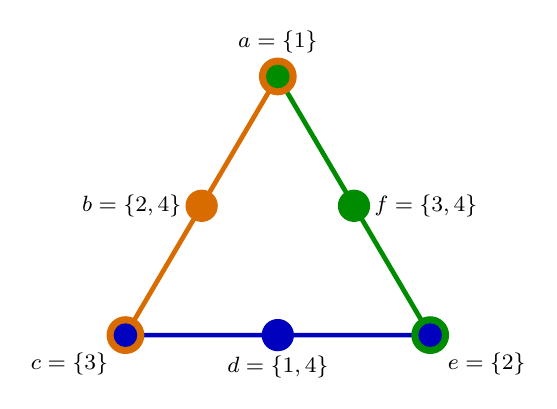
\begin{tikzpicture}[
  scale=0.9,
  outer vertex/.style={circle,minimum size=4.8mm,inner sep=0pt},
  inner vertex/.style={circle,minimum size=3.0mm,inner sep=0pt},
  single vertex/.style={circle,minimum size=4.1mm,inner sep=0pt},
  set label/.style={fill=white,inner sep=1.2pt,font=\footnotesize},
  orange context/.style={line width=1.7pt,orange!85!black},
  blue context/.style={line width=1.7pt,blue!75!black},
  green context/.style={line width=1.7pt,green!55!black}
]
\coordinate (A) at (0,2.5);
\coordinate (C) at (-2.15,-1.15);
\coordinate (E) at (2.15,-1.15);
\coordinate (B) at ($(A)!0.5!(C)$);
\coordinate (D) at ($(C)!0.5!(E)$);
\coordinate (F) at ($(E)!0.5!(A)$);
\draw[orange context] (A)--(B)--(C);
\draw[blue context] (C)--(D)--(E);
\draw[green context] (E)--(F)--(A);

% Shared corner outcomes are shown as concentric context colours.
\node[outer vertex,fill=orange!85!black,
  label={[set label]above:$a=\{1\}$}] at (A) {};
\node[inner vertex,fill=green!55!black] at (A) {};
\node[outer vertex,fill=orange!85!black,
  label={[set label]below left:$c=\{3\}$}] at (C) {};
\node[inner vertex,fill=blue!75!black] at (C) {};
\node[outer vertex,fill=green!55!black,
  label={[set label]below right:$e=\{2\}$}] at (E) {};
\node[inner vertex,fill=blue!75!black] at (E) {};

\node[single vertex,fill=orange!85!black,
  label={[set label]left:$b=\{2,4\}$}] at (B) {};
\node[single vertex,fill=blue!75!black,
  label={[set label]below:$d=\{1,4\}$}] at (D) {};
\node[single vertex,fill=green!55!black,
  label={[set label]right:$f=\{3,4\}$}] at (F) {};
\end{tikzpicture}
\caption{The three-uniform triangle test hypergraph.  Each colored side is one
designated three-outcome context; concentric colors mark outcomes shared by two
contexts.  The corner vertices $a,c,e$ are pairwise exclusive, although
$\{a,c,e\}$ is not one of the designated partitions.}
\label{fig:triangle}
\end{figure}

\subsection{A valid partition model with extra cross-context order}

Equation~\eqref{eq:triangle-partitions} is already a concrete partition
representation.  It also reveals relations not visible in
Fig.~\ref{fig:triangle}:
\begin{align}
  e=\{2\}&\subset b=\{2,4\},\nonumber\\
  a=\{1\}&\subset d=\{1,4\},\label{eq:triangle-inclusions}\\
  c=\{3\}&\subset f=\{3,4\}.\nonumber
\end{align}
Thus all six vertices are atoms of their local three-element partitions, but
only $a,c,e$ are singleton atoms in the global Boolean algebra $2^S$.  Reading
the drawing as an abstract Greechie diagram of six global atoms would therefore
produce a different ordered object from the concrete subset logic.

Furthermore, $a,c,e$ occur pairwise in the three different contexts, so the
orthoset obtained from Eq.~\eqref{eq:test-orthogonality} regards them as a
pairwise orthogonal triple.  Within the six-vertex orthoset it is maximal, even
though it was not stipulated as a complete test.  Pairwise exclusivity has
therefore generated a fourth ``phantom context.''  In the underlying set model,
$a\cup c\cup e=\{1,2,3\}$ leaves the case $4$ unaccounted for; the triple is
jointly disjoint but is not a partition of $S$.

\subsection{A general rank obstruction and the triangle}

The incidence pattern in Fig.~\ref{fig:triangle} is a loop of order three.
Such a loop is excluded from a Greechie diagram representing an orthomodular
poset; loops of order four mark the corresponding obstruction to the lattice
property.  These short-loop phenomena and their Hilbert-lattice realizability
have long been part of the pasting literature
\cite{greechie:71,svozil-tkadlec}.  The following elementary proposition does
not claim a new loop lemma.  It isolates the dimension-theoretic mechanism in
orthoset language and states the resulting obstruction for arbitrary rank.

\begin{proposition}[Unique-complement obstruction]
\label{prop:unique-complement}
Suppose that an exclusivity structure $(X,\perp)$ contains a pairwise
orthogonal set $B=\{x_1,\ldots,x_n\}$.  Suppose also that for
some $j$ there is a point $y\notin B$ satisfying
\begin{equation}
  y\perp x_i\qquad\text{for every }i\ne j.
  \label{eq:unique-complement-pattern}
\end{equation}
Then no assignment of distinct rays to the points of $X$ in an
$n$-dimensional anisotropic Hermitian space can preserve all the stated
orthogonalities.
\end{proposition}

\begin{proof}
The images of $x_1,\ldots,x_n$ are $n$ mutually orthogonal rays and hence form
an orthogonal basis spanning the entire $n$-dimensional space.  The orthogonal
complement of the span of $\{x_i:i\ne j\}$ is therefore the one-dimensional
subspace represented by the ray $x_j$.  Condition
\eqref{eq:unique-complement-pattern} forces the nonzero image of $y$ into that
same one-dimensional subspace, so the image rays of $y$ and $x_j$ coincide.
Because $y\notin B$, this contradicts faithfulness.
\end{proof}

Equivalently, a necessary combinatorial condition for faithful rank-$n$
realizability is that no vertex outside an orthogonal $n$-clique have all
$n-1$ vertices of one of its codimension-one faces as neighbours.  The
condition is only necessary; passing it does not guarantee a global vector
realization.

\begin{corollary}[Triangle obstruction]
There is no assignment of six distinct projective points of a
three-dimensional anisotropic Hermitian space to the vertices in
Eq.~\eqref{eq:triangle-contexts} that preserves the pairwise orthogonalities
within the displayed contexts.
\end{corollary}

\begin{proof}
The displayed contexts imply
\begin{equation}
  a\perp c,\qquad c\perp e,\qquad e\perp a,
  \label{eq:corner-orthogonality}
\end{equation}
so $B=\{a,c,e\}$ is an orthogonal triple.  The vertex $b\notin B$ is
orthogonal to $a$ and $c$, and Proposition~\ref{prop:unique-complement}
forces $b=e$.  Cyclically, the same argument gives
\begin{equation}
  b=e,\qquad d=a,\qquad f=c.
  \label{eq:triangle-collapse}
\end{equation}
Thus the representation is not faithful.
\end{proof}

Only anisotropy and dimension enter this argument, not a specifically real or
complex scalar field.  The class of finite partition test hypergraphs is
therefore not contained in the class of finite ray test hypergraphs faithfully
realizable at the same rank.

\subsection{What representations remain possible?}

First, the exclusivity graph does have a faithful ray representation already in
$\mathbb R^4$, and hence also after complexification.  With
$e_1,\ldots,e_4$ the standard basis, take
\begin{align}
 a&=e_1,& b&=\tfrac1{\sqrt2}(e_2+e_4),& c&=e_3,\nonumber\\
 d&=\tfrac1{\sqrt2}(e_1+e_4),& e&=e_2,&
 f&=\tfrac1{\sqrt2}(e_3+e_4).
 \label{eq:triangle-rays-four}
\end{align}
Each displayed triple is orthonormal, and among these six rays orthogonality
occurs exactly for pairs joined within a displayed context.  But the triples are
not complete bases of $\mathbb R^4$; each lacks a fourth ray.  Hence this is a
faithful representation of the graph as a finite fragment, not a realization
of the three hyperedges as complete rank-one contexts.

The missing rays can be adjoined explicitly:
\begin{equation}
\begin{aligned}
  g&=\tfrac1{\sqrt2}(e_2-e_4),&
  h&=\tfrac1{\sqrt2}(e_1-e_4),\\
  k&=\tfrac1{\sqrt2}(e_3-e_4).&&
\end{aligned}
  \label{eq:triangle-completing-rays}
\end{equation}
Then
\begin{equation}
 \{a,b,c,g\},\qquad \{c,d,e,h\},\qquad \{e,f,a,k\}
 \label{eq:triangle-completed-contexts}
\end{equation}
are orthonormal bases of $\mathbb R^4$.  This is a genuine enlargement of the
test hypergraph: each original three-outcome test becomes a proper subset of a
new four-outcome test.  It does not turn the original triples into complete
three-outcome contexts.

Second, Eq.~\eqref{eq:diagonal-projection} gives a complete projection-valued
representation in $\mathbb C^4$:
\begin{align}
 \pi_1&:\quad P_{\{1\}}+P_{\{2,4\}}+P_{\{3\}}=I,\nonumber\\
 \pi_2&:\quad P_{\{3\}}+P_{\{1,4\}}+P_{\{2\}}=I,\label{eq:triangle-pvms}\\
 \pi_3&:\quad P_{\{2\}}+P_{\{3,4\}}+P_{\{1\}}=I.\nonumber
\end{align}
One projector in each row has rank two.  All six projectors commute because
they are diagonal in the same basis.  Together with the ray construction, this
gives the following qualified statement:
\begin{quote}
The triangle occurs as a finite commuting projection configuration, and its
exclusivity graph occurs as an incomplete ray configuration in dimension four
that can be enlarged to four-outcome bases; it does not occur faithfully as
three rank-three ray contexts.
\end{quote}

\section{Finiteness: obstruction, boundary, and completion}
\label{sec:finiteness}

Two uses of the word ``finite'' must be separated:
\begin{enumerate}
\item \emph{finite rank}: at most $n$ mutually orthogonal points exist;
\item \emph{finite cardinality}: the total point set $X$ is finite.
\end{enumerate}
A finite-dimensional real or complex Hilbert space has finite rank but
infinitely many rays.  Thus finite rank never implies a finite modality or
point set.

The finite analysis of Emir, Kruml, Paseka, and Vetterlein, and its later
extensions, yields a sharp fact: a linear orthoset of rank at least three is
infinite \cite{EmirKrumlPasekaVetterlein2021,
EmirPasekaVetterlein2023Finitary}.  Finite rank-two linear orthosets reduce to
orthogonal pairings, while finite rank-three structures can satisfy weaker
prelinearity properties but not full linearity.

Therefore a finite partition logic of rank at least three cannot itself be the
entire linear orthoset $\Proj(H)$.  This is consistent with the scope of the
representation theorem: a finite contextual structure can at most be a
fragment or a structure to be completed.  The completion must add enough points
to populate projective lines and satisfy the global replacement axiom.

Three further consequences clarify this boundary.

First, completion is substantive, not merely a change of notation.  If
$X\subset\Proj(H)$ is finite, then the internal closure
\begin{equation}
  \{e,f\}^{\perp_X\perp_X}
  \label{eq:internal-closure}
\end{equation}
can be much smaller than the full projective line
$\Proj(\Span(e,f))$.  Adding the missing points changes the orthoclosed-event
structure.

Second, orthogonality data need not determine a unique completion unless the
projective and symmetry axioms required by the representation theorem are
assumed.  Even after a generalized Hermitian space is obtained, the scalar
division ring need not be $\mathbb C$.

Third, finiteness alone does not distinguish classical from quantum
representability.  Every finite partition model embeds diagonally into a finite
complex Hilbert space, while only some exclusivity graphs admit faithful ray
representations in a prescribed low dimension.  What finiteness obstructs is
the identification of the finite structure with a \emph{complete linear
projective orthoset} of rank at least three.

\section{States and probabilities}
\label{sec:probability}

Neither a test hypergraph nor an orthogonality graph uniquely fixes its state
space.  A partition representation supplies a natural classical choice.  If
$\lambda_s\ge0$ and $\sum_s\lambda_s=1$, then
\begin{equation}
  p(A)=\sum_{s\in A}\lambda_s
  \label{eq:classical-probability}
\end{equation}
is additive on every partition context.  These probabilities form the convex
hull of the two-valued evaluations in Eq.~\eqref{eq:valuation}.

A ray representation supplies a different possible resource.  Given a unit
state vector $\psi$ and ray projectors $P_x$, one may define
\begin{equation}
  p_\psi(x)=\langle\psi,P_x\psi\rangle.
  \label{eq:born-weight}
\end{equation}
For a complete orthonormal basis the weights sum to one.  Gleason's theorem
shows, in Hilbert-space dimension at least three and under its additivity
hypotheses on the full Hilbert lattice, how density operators characterize such measures
\cite{Gleason}.  But Eq.~\eqref{eq:born-weight} uses structure not contained in
an arbitrary finite graph: a chosen scalar field, inner product, complete
contexts, and a state.

This is why one finite exclusivity graph may support both a classical partition
model and a quantum vector model with different convex sets of probabilities
\cite{svozil-2018-b}.  Orthogonality is a constraint on joint zero transition
probabilities; it is not by itself the Born rule.

The basic linear-orthoset theorem likewise does not reconstruct mixed states,
tensor products, composition of systems, time evolution, observable algebras,
or operational continuity.  Those may be introduced or characterized in richer
frameworks; they are additional structures rather than consequences of the bare
orthogonality relation.

\section{Structural implications and scope}
\label{sec:claims}

The comparison supports the following affirmative statements.

\begin{enumerate}
\item Partition logics and orthosets share a combinatorial core of elementary
outcomes and exclusivity.
\item A partition test space produces an orthoset by forgetting all but
pairwise exclusivity witnessed within tests.
\item The layered structure $(X,\perp,\cE)$ can preserve both exclusivity and
designated complete tests; enlarging $\cE$ systematically restricts the
admissible state space.
\item A finite test hypergraph is faithfully partition-representable exactly
when it has a nonzero separating family of admissible two-valued states.
\item Some partition exclusivity graphs possess faithful orthogonal vector
representations; the same graph can consequently admit distinct physical and
probabilistic realizations.
\item Vetterlein's linearity axiom identifies when orthogonality is rich enough
to recover projective span and generalized Hermitian geometry at rank at least
four.
\item Additional automorphism axioms can substantially restrict the allowed
Hermitian or quadratic spaces.
\end{enumerate}

The corresponding scope distinctions are as follows.

\begin{enumerate}
\item Overlapping or ``intertwining'' contexts alone do not imply linearity.
\item The exclusivity graph does not retain the complete-test hypergraph in
general.
\item Declaring every maximal orthogonal set complete is an additional
postulate and can eliminate states inherited from the partition carrier.
Orthogonal closure, test saturation, and projective point completion are
distinct operations.
\item The unique-complement obstruction in
Proposition~\ref{prop:unique-complement} is a necessary condition for faithful
rank-$n$ ray realizability; the three-loop triangle violates it.
\item A Kochen--Specker-uncolourable test hypergraph cannot be a partition
logic, because it lacks even one admissible two-valued state.
\item A finite partition logic of rank at least three cannot equal a full linear
orthoset, because such a linear orthoset must be infinite.
\item A generalized anisotropic Hermitian space is not automatically a real or
complex Hilbert space.
\item The Hilbert-field minimality theorem gives a countable dense real
subgeometry that embeds in every quadratic orthoset of the same finite rank; it
does not give equality with real or complex projective Hilbert space.
\item Orthogonality and its automorphisms alone do not automatically provide
the complete probabilistic and dynamical formalism of quantum mechanics.
\end{enumerate}

In this manuscript, ``reconstruction'' refers to a representation or
characterisation theorem: a relational structure satisfying specified strong
axioms is shown to be isomorphic to the projective orthogonality structure of a
member of a stated class of inner-product spaces.  The operational motivation
of the axioms, selection of a scalar field, and construction of the remaining
quantum formalism are further questions beyond that representation statement.

\section{Conclusion}
\label{sec:conclusion}

Partition logics and linear orthosets begin near the same operational image---a
collection of experimental alternatives grouped into mutually exclusive
contexts---but travel in opposite mathematical directions.  Partition logic
adds a finite classical carrier beneath the contexts.  Vetterlein's programme
removes almost everything except orthogonality and then imposes sufficiently
strong global regularity to recover projective geometry.

An intermediate test-orthoset layer makes a controlled interpolation possible.
It preserves a set of outcomes, their pairwise exclusivity, and a separately
designated family of complete tests.  Saturating that family adds normalization
conditions and restricts admissible states; closing under $\perp\perp$ builds a
new event lattice; adjoining points to enforce linearity seeks a genuinely
projective completion.  These three enlargements answer different questions.

The relation is therefore neither identity nor disjointness.  A finite
partition logic can supply the same exclusivity skeleton as a finite fragment
of a Hermitian projective geometry, and it always has a diagonal representation
by commuting Hilbert-space projections.  Yet partition logics can also contain
test structures, such as the three-uniform triangle, that cannot be interpreted
faithfully by distinct rays at the corresponding rank.  The general
unique-complement obstruction identifies one combinatorial source of such
failures.  Conversely, the separating-state criterion identifies exactly when
a finite test hypergraph has a faithful partition representation.  When only
pairwise orthogonality is retained, even the stipulated set of tests may change.

Conversely, a full projective orthoset is vastly richer than a finite pasted
family of tests.  Its lines are saturated, its orthogonal closure determines
projective span, and at rank at least three its linearity forces infinitely many
points.  Rank four enters because it is the general coordinatization threshold.
Symmetry conditions may then restrict the scalar system, with the outcome
depending on the hypotheses: an anisotropic Hermitian space, a real-type
quadratic space over an ordered or Pythagorean field, a Hilbert-field
subgeometry, or---under
stronger infinite-dimensional assumptions---a classical Hilbert space.

Thus finite partition logics are useful both as models and as diagnostic
comparison cases.  They show precisely which consequences follow from local
Booleanity and intertwining, and which require the global projective,
homogeneity, field, and completeness assumptions of a Hilbert-space
reconstruction.

\begin{acknowledgments}
\small
The author thanks Philippe Grangier for valuable discussions.

This research was funded in whole or in part by the Austrian Science Fund
(FWF) [Grant DOI:
\href{https://doi.org/10.55776/PIN5424624}{10.55776/PIN5424624}].  For open
access purposes, the author has applied a CC BY public copyright license to any
author accepted manuscript version arising from this submission.  The author
acknowledges TU Wien Bibliothek for financial support through its Open Access
Funding Programme.

OpenAI Codex (GPT-5) was used to assist with literature organization, \LaTeX{}
editing, and checks of derivations.  The author specified the scientific
direction and prompts; model output retained in the manuscript was checked
against the cited sources and explicit calculations.  The author accepts full
responsibility for the final text.
\end{acknowledgments}

\clearpage
\bibliography{svozil}

\end{document}
